\newpage
\phantomsection
\label{prf:euclid-i-46}
\LRAProofFor{thm:euclid-i-46}

\begin{remark*}[Return]
\hyperref[thm:euclid-i-46]{Return to Theorem}
\end{remark*}

\begin{theorem*}[Euclid I.46: Constructing a square on a segment]
On a given straight line, to describe a square.
\end{theorem*}

\begin{center}
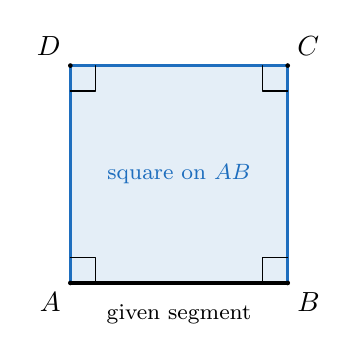
\begin{tikzpicture}[scale=1.15, line cap=round, line join=round]
  \definecolor{euclidblue}{RGB}{30,110,190}
  \coordinate (A) at (0,0);
  \coordinate (B) at (2.4,0);
  \coordinate (C) at (2.4,2.4);
  \coordinate (D) at (0,2.4);
  \fill[euclidblue!12] (A)--(B)--(C)--(D)--cycle;
  \draw[very thick, euclidblue] (A)--(B)--(C)--(D)--cycle;
  \draw[very thick] (A)--(B);
  \draw (0.28,0)--(0.28,0.28)--(0,0.28);
  \draw (2.12,0)--(2.12,0.28)--(2.4,0.28);
  \draw (2.12,2.4)--(2.12,2.12)--(2.4,2.12);
  \draw (0.28,2.4)--(0.28,2.12)--(0,2.12);
  \foreach \p/\pos in {A/below left,B/below right,C/above right,D/above left}{
    \fill (\p) circle (0.026);
    \node[\pos] at (\p) {$\p$};
  }
  \node[font=\footnotesize] at (1.2,-0.35) {given segment};
  \node[euclidblue, font=\footnotesize] at (1.2,1.2) {square on $AB$};
\end{tikzpicture}
\end{center}


\begin{proof}[Professional Standard Proof]
\LRAProofBodyStart
Let $AB$ be the given segment. At $A$, draw a perpendicular to $AB$ and cut off
$AD$ equal to $AB$. Through $D$, draw a line parallel to $AB$; through $B$,
draw a line parallel to $AD$. Let those two parallels meet at $C$.

The quadrilateral $ABCD$ has opposite sides parallel, so it is a parallelogram.
The construction gives one right angle, and the parallel lines transfer right
angles to the remaining corners. Also $AD=AB$ by construction, and opposite
sides of the parallelogram are equal. Thus all four sides are equal and all
four angles are right angles. By the definition of a square, $ABCD$ is the
square on $AB$.
\end{proof}

\begin{proof}[Detailed Learning Proof]
\LRAProofBodyStart
The construction first creates one side perpendicular to the given segment and
equal to it. The two parallels then close the quadrilateral without changing
the directions: horizontal sides stay parallel to $AB$, and vertical sides stay
parallel to $AD$. This makes a right-angled parallelogram whose adjacent sides
are equal, hence a square.
\end{proof}

\begin{remark*}[Proof structure]
Construct a perpendicular equal side, close the figure with parallels, and use
parallel transfer of right angles plus equality of opposite sides to identify a
square.
\end{remark*}

\begin{dependencies}
\begin{itemize}
  \item \hyperref[def:euclid-quadrilateral-classes]{Square}
  \item \hyperref[thm:euclid-i-31]{Euclid I.31}
  \item \hyperref[ax:euclid-postulate-draw-straight-line]{Euclid Postulate I}
  \item \hyperref[ax:euclid-postulate-right-angles-equal]{Euclid Postulate IV}
\end{itemize}
\end{dependencies}

\clearpage
